\documentclass{beamer}
\usetheme{Madrid}
\usepackage{lmodern}% http://ctan.org/pkg/lm
\setbeamersize{text margin left = 2.5em}
\setbeamersize{text margin right = 2.5em}
\usepackage{color}
\usepackage{graphicx}
\usepackage{MnSymbol}
\usepackage{amsmath}
\usepackage{comment}
\usepackage{tikz}
\usepackage{subfigure}
\usepackage{listings}
\usetikzlibrary{automata}

%\usepackage[backend=bibtex,sorting=none]{biblatex}
%\addbibresource{E:/Papers/LiuLab} %BibTeX�����ļ���λ��
%\setbeamerfont{footnote}{size=\tiny}
\setbeamertemplate{theorems}[numbered]
\setbeamertemplate{caption}[numbered]
%% ʹ�ý�ע���õ�Ƭijҳ���Ӳο����ס�
%% ��������ʹ�ã�\footfullcite{bib_item} %����item
%% \usepackage{anyfontsize}%% allowing font sizes at arbitrary sizes
\logo{
\includegraphics[height=0.05\textwidth]{Pic/logo}}
\newtheorem{df}{Definition}
\newtheorem{DF}{DEFINITION}
\newtheorem{prop}{Proposition}
\newtheorem{thm}{Theorem}
\newtheorem{cor}{COROLLARY}
\newtheorem{lm}{LEMMA}
% ----------------------------------------------------------------------------------------
% TITLE PAGE
% ----------------------------------------------------------------------------------------

\title{E04 Futoshiki Puzzle (Forward Checking)}
% The short title appears at the bottom of every slide, the full title is only on the title page

\author{Suixin Ou} % Your name
\institute[SYSU] % Your institution as it will appear on the bottom of every slide, may be shorthand to save space
{
  School of Computer Science\\
  Sun Yat-sen University \\ % Your institution for the title page
  \medskip
  % Your email address
}

\date{October 12, 2021} % Date, can be changed to a custom date

\AtBeginSection[]
{
  \begin{frame}
    \tableofcontents[currentsection,currentsubsection]
  \end{frame}
}

\begin{document}

\begin{frame}
  \titlepage
\end{frame}

\begin{frame}
  \frametitle{Task}
  \begin{block}{Problem}
\begin{itemize}
    \item Futoshiki is a board-based puzzle game. It is playable on a square board having a given fixed size.

     \item The purpose of the game is to discover the digits hidden inside the board’s cells; each cell is filled with a digit between 1 and the board’s size. On each row and column each digit appears exactly once; therefore, when revealed, the digits of the board form a so-called Latin square.

   \item  At the beginning of the game some digits might be revealed. The board might also contain some inequalities between the board cells; these inequalities must be respected and can be used as clues in order to discover the remaining hidden digits.

   \item  Each puzzle is guaranteed to have a solution and only one.

    \item You can play this game online: http://www.futoshiki.org/.
    \end{itemize}
  \end{block}
\end{frame}





\begin{frame}
  \frametitle{Task}
  \begin{block}{Input-output}
    \begin{itemize}
      \item Input: a n x n matrix of initial state, and a list of inequal constraints.


	  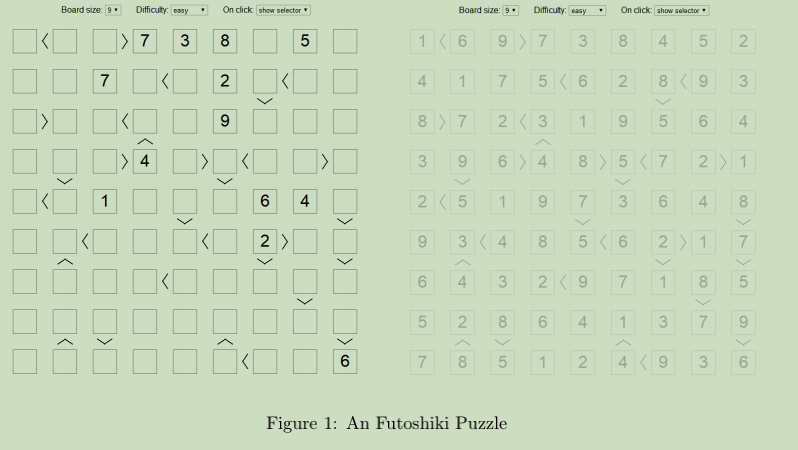
\includegraphics[width=0.7\textwidth]{Pic/figure1}

      \item Output: the n x n matrix of the terminate state that satisfys all constraints (including inequal constraints, row and column constraints).
    \end{itemize}
  \end{block}
\end{frame}
\begin{frame}

  \frametitle{Task}
  \begin{block}{Submission}
    pack your report \texttt{E04\_YourNumber.pdf} and source code into zip file \texttt{E04\_YourNumber.zip}, then send it to \texttt{ai\_course2021@163.com}.
  \end{block}
\end{frame}

\begin{frame}
  \frametitle{Solution}
  Algorithm procedure
  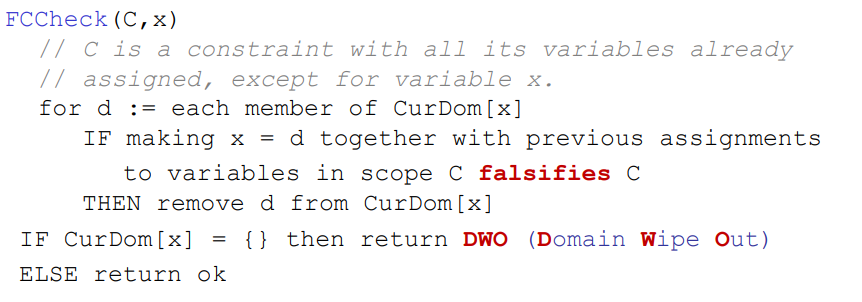
\includegraphics[width=0.8\textwidth]{Pic/fc1}
\end{frame}

\begin{frame}
  \frametitle{Solution}
  Algorithm procedure
  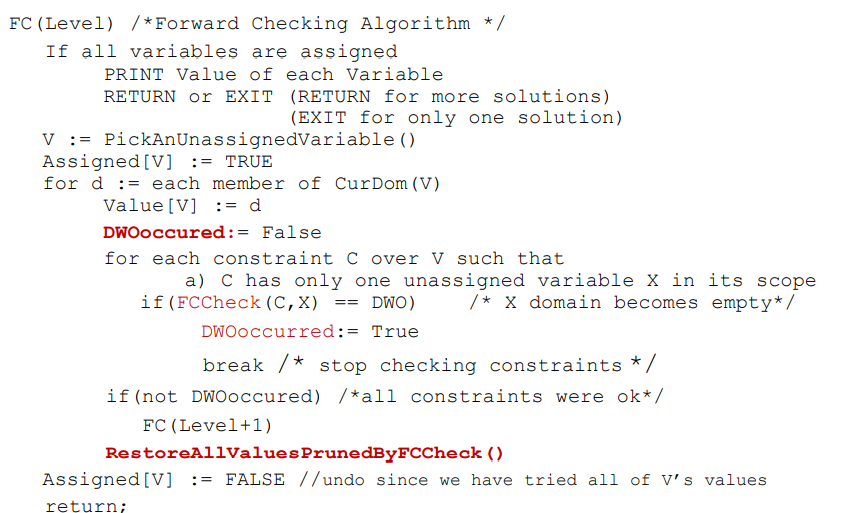
\includegraphics[width=0.8\textwidth]{Pic/fc2}
\end{frame}


\begin{frame}
  \frametitle{Solution}
  \begin{columns}
    \begin{column}{.5\linewidth}
      Read input
      
      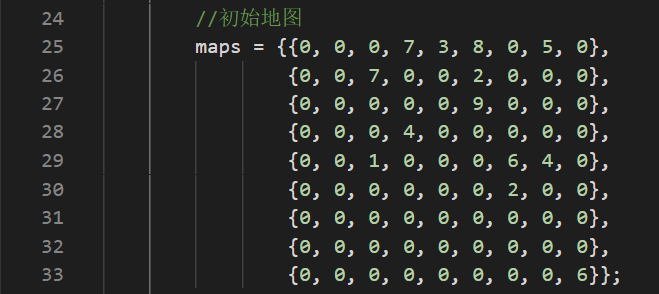
\includegraphics[width=1.05\textwidth]{Pic/ini}

      
      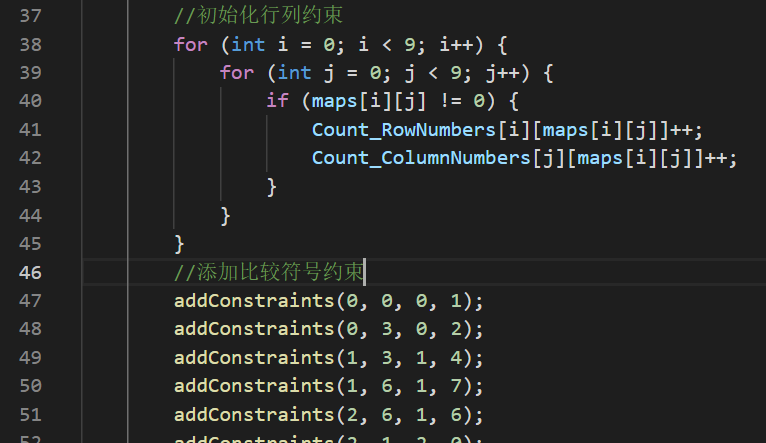
\includegraphics[width=1.05\textwidth]{Pic/addC}
    \end{column}
    \begin{column}{.5\linewidth}
      Visualize output
      
      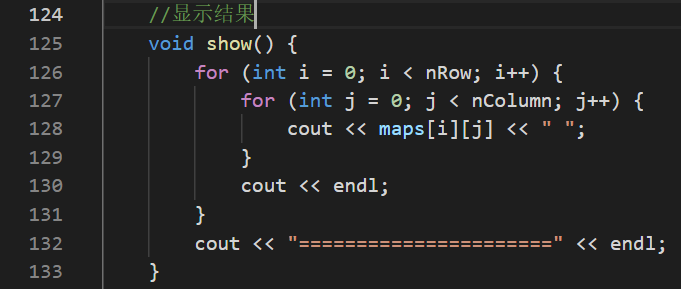
\includegraphics[width=1.05\textwidth]{Pic/print}
    \end{column}
  \end{columns}

\end{frame}

\begin{frame}
  \frametitle{Solution}
      Check whether conditions are all satisfied.
      \textbf{You should finish a check function for the Forward Checking algorithm.}
      
      
      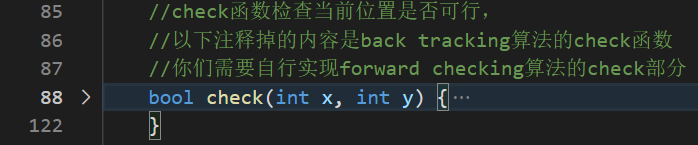
\includegraphics[width=.9\textwidth]{Pic/check}
      Search for correct solution.
      
      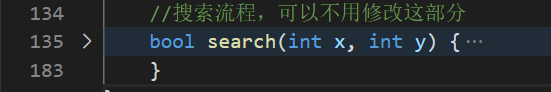
\includegraphics[width=.9\textwidth]{Pic/search}

\end{frame}


\begin{frame}
  \frametitle{Task}
  \begin{block}{Some discussion}
	  You are encouraged to explore(\textbf{not necessary}):
    \begin{itemize}
      \item Differences between back tracking and forward checking algorithm;
	  \item Influences introduced by the case difficulty;
	  \item Tradeoff between search expenses caused by the number of searched nodes and checking expenses caused by the constraint checking in every single node;
    \end{itemize}
  \end{block}
\end{frame}

%-----------------------------------------------------------------------------------------

\begin{frame}
  \Huge{\centerline{The End}}
\end{frame}

% ----------------------------------------------------------------------------------------


\end{document}
